\section{Tekniskt bidrag}% "Contributions" -- Syfte.
Med en budget på 5000 kr har ett system innehållande en robothand med tre fingrar som styrs trådlöst med en styrhandske utvecklats. Utifrån Cutkoskys grepphierarki, se Appendix\ref{cutshand}, utformas robothanden och dess fingrar för att möjliggöra ett stort antal olika grepp, med olika krav på styrka, omfång, finkänslighet och fingerfärdighet. Grunden till den mekaniska konstruktionen utgörs av Meccano med följden att delarna blir standardiserade och behovet att tillverka mekaniska delar kringgås. Totalt har robothanden åtta leder varav sex är separat styrbara och aktueras av varsin sevomotor. Robothandens fingrar har ett människolikt rörelsemönster för att användaren intuitivt skall kunna styra den med sina egna fingrar via styrhandsken.

För att styrhandsken skall passa olika händer kalibreras den enkelt av användaren själv med två knapptryckningar. I styrhandsken registrerar sex flexresistorer användarens fingerrörelser. Mätvärdena från dessa behandlas av en \emph{Arduino Micro} som sedan trådlöst kommunicerar med robothandens \emph{Arduino Due} där dessa används som styrsignaler till servomotorerna.\\ För att undvika skador på objekt mäter robothanden kontakttrycket med hjälp av trycksensorer på fingertopparna, vars mätvärden återkopplas till användaren via ledramper som lyser upp proportionerligt mot uppmätt tryck. För att ytterligare \comment{Här bryter vi tills vi vet om handen gör nåt eller bara följer fingrar. det unfer är old som nog kan användas}
Vidare krävs stabila styrsignaler från styrhandsken till robothanden som utnyttjas på ett bra sätt för att åstadkomma god åtföljning. Detta uppnås genom designade butterworthfilter och programmering. För att användare med olika handstorlek ska uppleva god åtföljning vid styrning är det nödvändigt att kalibrera handsken för varje ny användare. Kalibreringenen sker enkelt med hjälp av två knappar som sitter på handskens kretskort. (Detta är något vi tillfört som är nytt va? Jag har inte läst om det nånstans...)

För att undvika skador på objekt som robothanden hanterar implementeras ett bibliotek av olika objekt i robothandens mikrokontroller som möjliggör objektidentifiering. Varje objekt har ett fördefinierat högsta tryck som robothanden får utsätta den för. Om operatören försöker greppa hårdare än det fördefinierade trycket reglerar robothanden detta för att undvika skada. Objektidentifieringen är baserad på igenkänning av objektets storlek genom att, utifrån vinklar på de styrande servomotorerna, beräkna avståndet mellan de tryckbelastade punkterna på robotfingrarna. Robothanden är försedd med endast tre trycksensorer vilket avsevärt begränsar antal grepp som möjliggör objektidentifiering. Vid greppning av objekt som inte är definierade i robothandens bibliotek kan användaren ändå få en uppfattning av trycket då det representeras av dioder på styrhansken. Högre tryck ger fler lyssande dioder.
Robothanden följer användarens fingerrörelser tills dess att den greppar ett av flera fördefinerade, kända objekt, då den istället verkar för att hålla objektet med en önskad kraft, tills dess att användaren visar att den vill släppa objektet igen genom att öppna sin hand. Nedan visas ett flödesschema för överskådligt beskriva hur robothanden principiellt fungerar.


Robothanden följer användarens fingerrörelser tills dess att den greppar ett av flera fördefinerade, kända objekt, då den istället verkar för att hålla objektet med en önskad kraft, tills dess att användaren visar att den vill släppa objektet igen genom att öppna sin hand. Nedan visas ett flödesschema för överskådligt beskriva hur robothanden principiellt fungerar.

\begin{figure}[H]
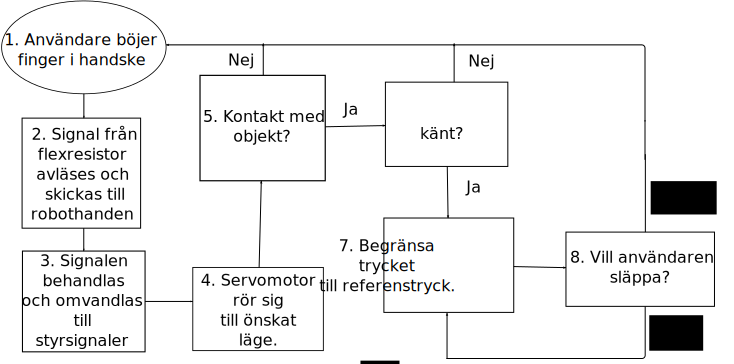
\includegraphics[width=.90\textwidth]{img/flodesschema}
\caption{Flödesschema över en tänkt signals väg genom robothanden.
\comment{det borde inte stå ändringen etc. det är inget som registrerar ``ändringar'' per se, signalen bearbetas kontinuerligt med eller utan ändringar}}
\label{flodesschema}
\end{figure}

\begin{enumerate}
\item Önskat fingerläge ges genom att användaren böjer sitt finger i kontrollhandsken.
\item Flexresistor på kontrollhandsken ändrar resistans.
\item Den ändrade resistansen avläses av en Arduino Micro enhet på kontrollhandsken som skickar den via bluetooth till en Arduino Mega enhet på robothanden.
\item Värdet på resistansen omvandlas till PWM-signal som kalibrerats av användaren vid uppstart.
\item PWM-signaler matas till aktuatorer som ställer sig i önskad vinkel.
\item Feedback från trycksensorer avläses och leder till ett stopp av aktueringen om avläst tryck är högre än fördefinerad gräns.
\end{enumerate}
Robothanden kan delas in i tre delsystem som samverkar för att uppfylla handens funktion. Delsystemen är styrhandske, styrsystem och robothand. Användaren har på sig styrhandsken och styrsystemet verkar för att robothanden ska imitera användarens fingerrörelser tills dess att robothanden kommer i kontakt med ett objekt.



%Detta är just nu en förklaring på vårt systems funktion bara. Bör ingå mer tekniskt? Vilka medel vi använt o så.